\chapter{PKG Ecosystem}
- A PKG Tool criteria must work with a graph or database and allow unrestricted linking of entities
    - otherwise it’s just KM Tool

\textbf{The prototype is about UI and UX, not PKG Ecosystem feature showdown!}

\begin{figure}
    \centering
    \label{fig:nink}
    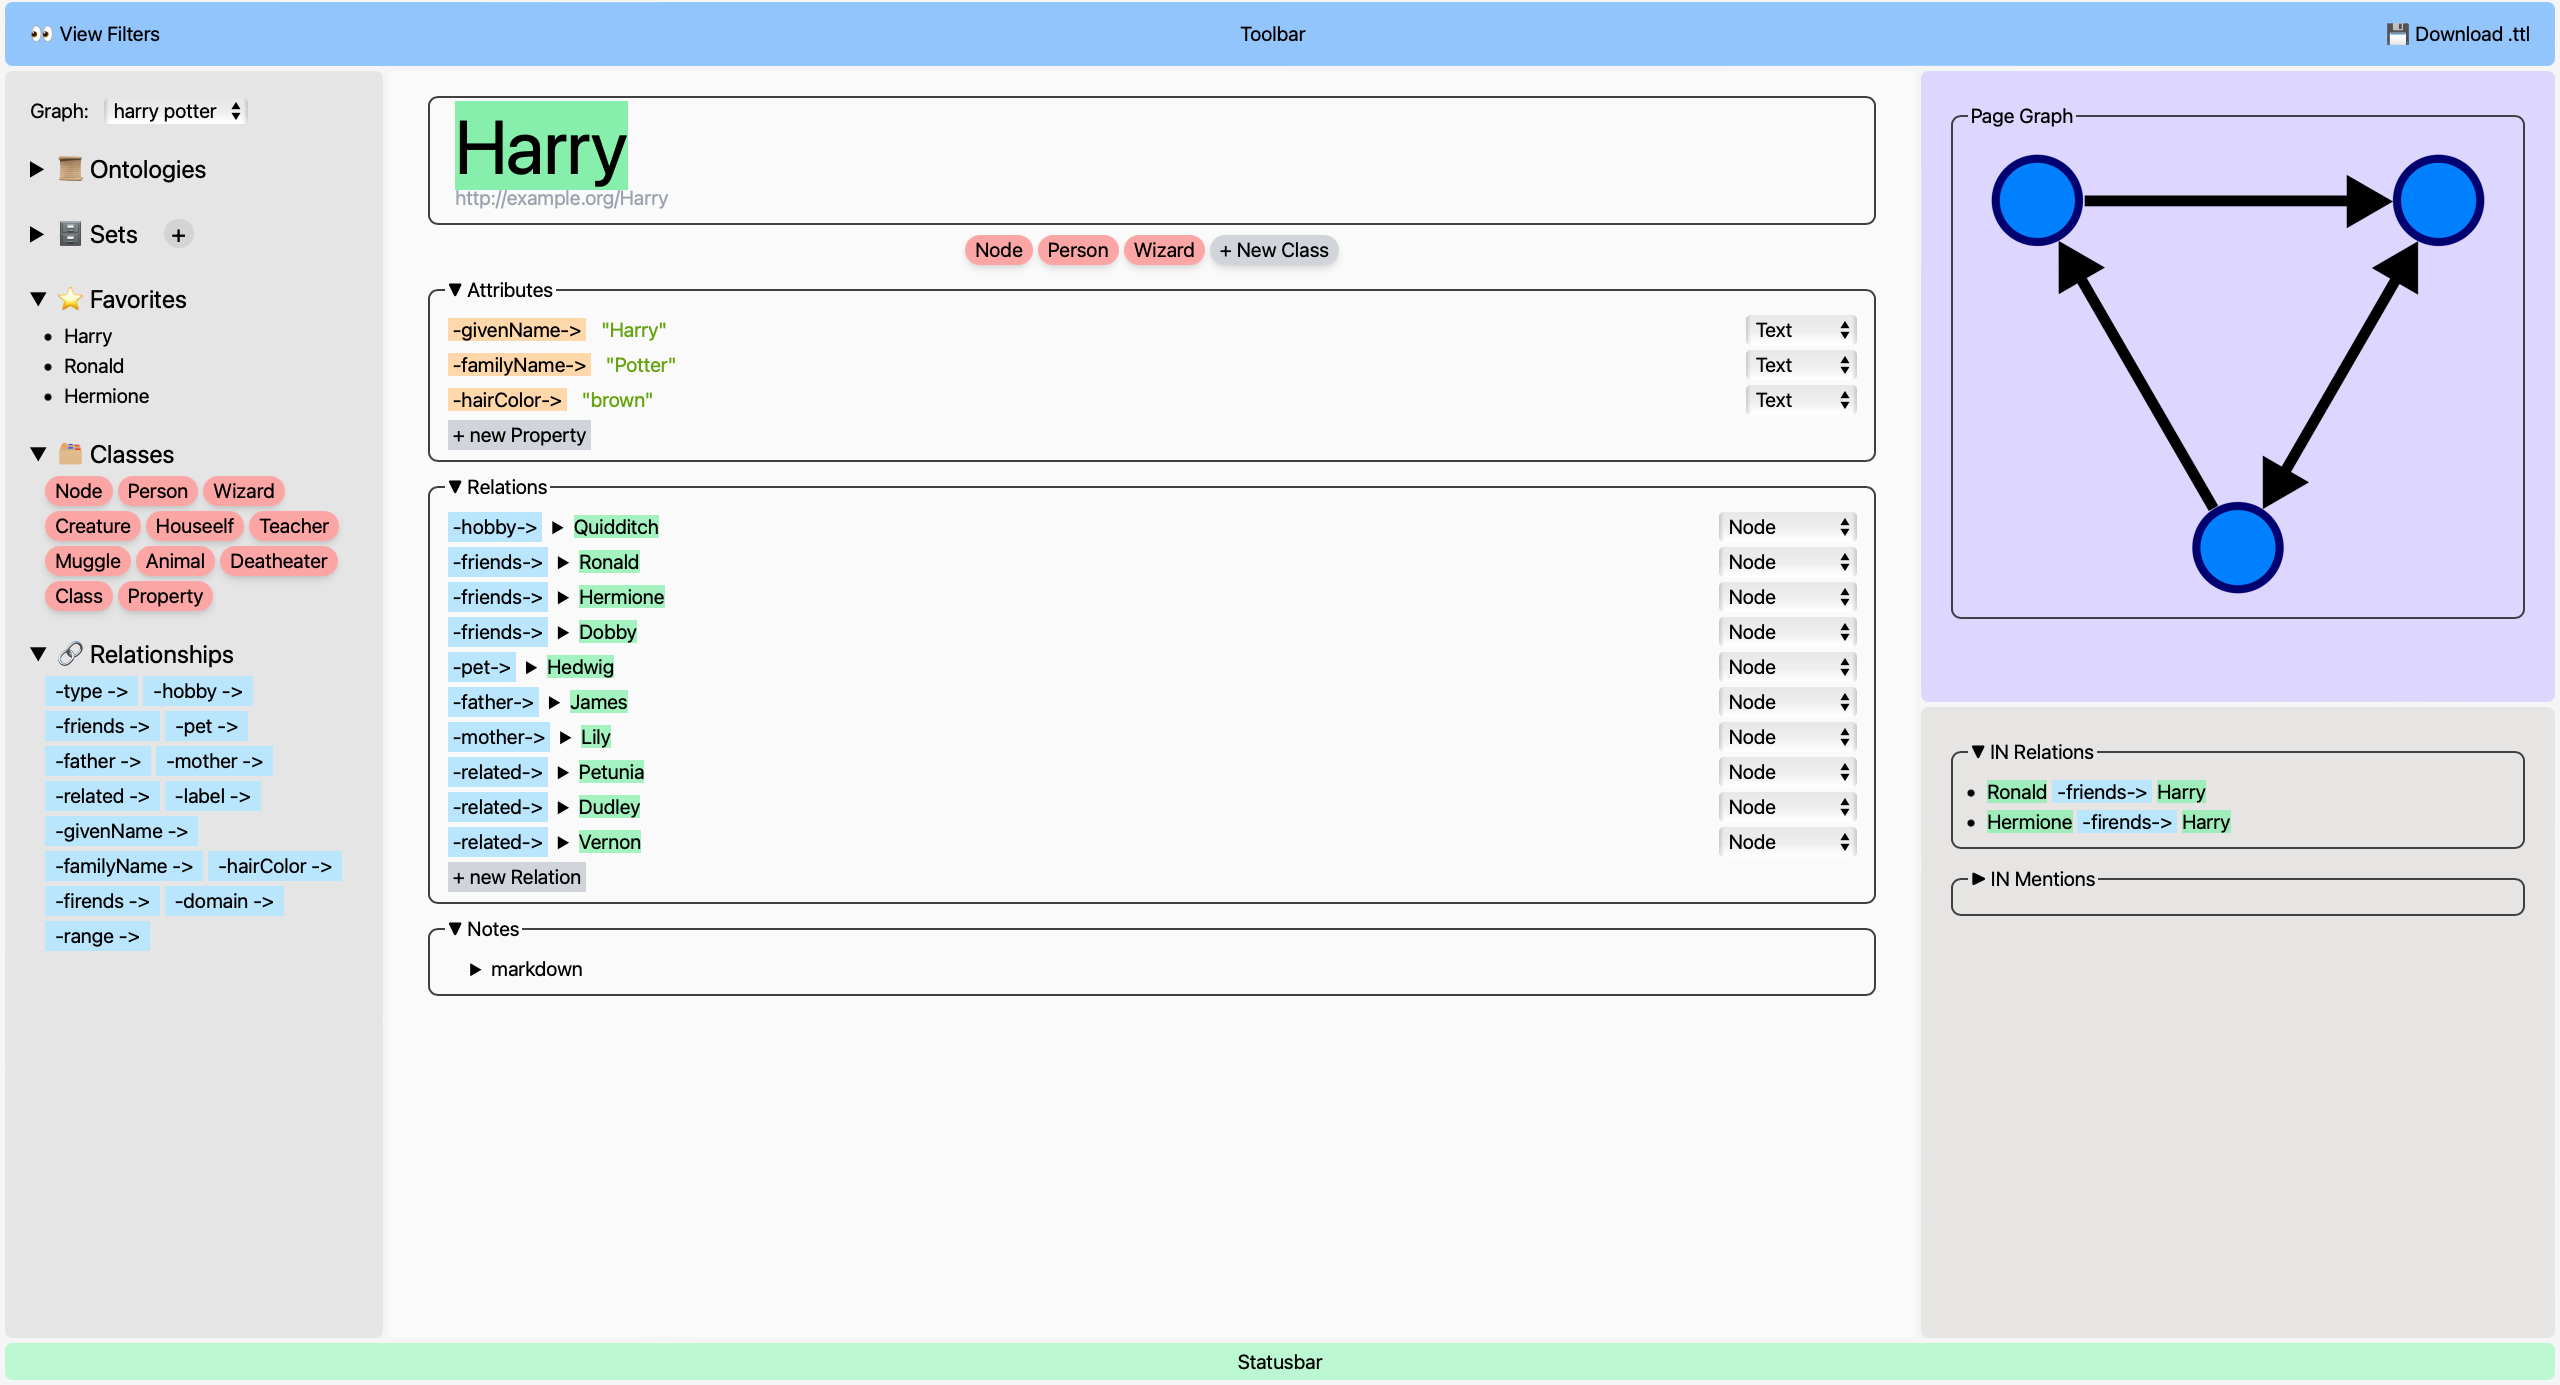
\includegraphics[width=\textwidth]{nink}
    \caption[short cap]{long caption}
\end{figure}
\section{Requirements for a PKG App Ecosystem}
- memex 60 years later **must have** functionality
- and everything from yourself
\section{Analysis of the Software Landscape}
- include current State of PKM
- web app, to reduce UX friction of install, login etc
- reference to other PKB Tools
- what basic features are needed?
    - bi-links
    - sets
    - overview of
        - in/out arcs
        - in/out mentions
- what are advanced features the model is capable of and could be explored?
- even though a prototype was implemented on SWS compatible Graph structure, that was more to showcase how easily implemented these features are on a real graph structure, and to show hard to understand SWS Concepts can be abstracted away.

Include all algorithms from code? how things are inserted into triple store etc?

- required structure of Data:
    - define what a Node is (Class Node?)
    - define what a Title is (Literal Label?)
\section{Applying the Model}
\section{Abstracting away Technical Details of Semantic Web Technologies}
\section{Testing Usability}


\section{unsorted}
current note taking tools only save “snapshots” of files in themselves, while we need the actual files (audio, video, pdf, text etc) to be workable and openable in any program. pkg needs to be a file system / cloud drive

Knowledge Graph Summarization: store only what’s relevant to the user

Premise Pkg stored in a cloud. Like social media posts or cloud drives, set visibility in the graph

integration of external knowledge by clicking add node / triple on external RDF data

**Abstract 0.1**

Semantic Web Technologies have been slow to adopt / gain traction outside of the academic areas. While there are relevant use cases in the industry, they are living a nieche dasein and are a tough sell. the lack of education and accessible tools for SWT means these technologies don’t get the spread necessary to really be usable and enable a semantic Web experience. This leads to SWT being sparely used on the internet, with the userbase being mostly academics, and sparcely in the industry.

This paper presents the implementation of a tool that tackles the problem of making a Tool (Broser Extension) that makes SWT approachable to the layman internet user. The hope is, that such a tool can drive adoption through implementation in Browsers, creating awareness of the technology and it’s benefits for regular people and the industry.

To be able to reach laymans, the software needs to have exceptionally easy UX and availability.

This means:

- no installation process
- no required configuration / setup
- no prior knowledge about the technologys and terms involved

To achieve these goals, the optimal case would be for Semantic Web Technologies to be integrated into browsers as a feature. Just like users are able to interact with websites now, in the future they should be able to browse and enrich / extend the semantic web.

Semantic Web Technologies, should be embedded into browsers, the same as features like having tabs, creating bookmarks, password managers or having a history visualization.

we will explore the matured state of these ideas due to evolution through time, as well as through the removal of technical hurdles.

We are building a web app, for usability sake, but also because semantic web is about WEB

When **loading RDF into a human readable editor, you get a load of machine relevant meta crap**

- Knowledge Graph Summarization: store only what’s relevant to the user

